\documentclass[10pt]{examdesign}
\usepackage{amsmath}
\usepackage{enumitem}
\usepackage{amsfonts}
\usepackage{pgfplots}
\usepackage{pifont}
\usepackage{graphicx}
\usepackage{fancyhdr}
\usepackage{cancel}
\usepackage{gensymb}
\usepackage[american]{circuitikz}

\SectionFont{\large\sffamily}
\Fullpages
\ContinuousNumbering
\usepackage{ulem}
\ProportionalBlanks{2}


\DefineAnswerWrapper{}{}
\NumberOfVersions{1}
%\IncludeFromFile{foobar.tex}
\examname{\Large{Centripetal Force and Acceleration}}
\class {\Large Physics}

\def \namedata {Name: \hrulefill\\ 
	Date: \hrulefill \\
	Period: \hrulefill \\
	Primary Peer Reviewer: \hrulefill 
	\\
			\begin{tabular}{| p{1cm} | p{1cm} | p{1 cm} | p{1cm} |}
	\hline
		+1 & 0 & -1 & $\Sigma$ 
		\\
		\hline
		& & & \vspace{.5cm}
		\\ \hline
	
	\end{tabular}
	\\
 \vspace{-.6in}
	
}




\begin{document}




\begin{multiplechoice} [title={Multiple Choice},
	rearrange=no]

\textit{For Each question, choose the best answer.}

	Some Formulas: 
	\begin{center}
	$F_c = \frac{mv^2}{r} $	\hspace{1 in} $a_c = \frac{v^2}{r}$ \hspace{1in} $c = 2 \pi r $
	\vspace{0.1in}
\end{center}	
	


\begin{question}
	\begin{center}
		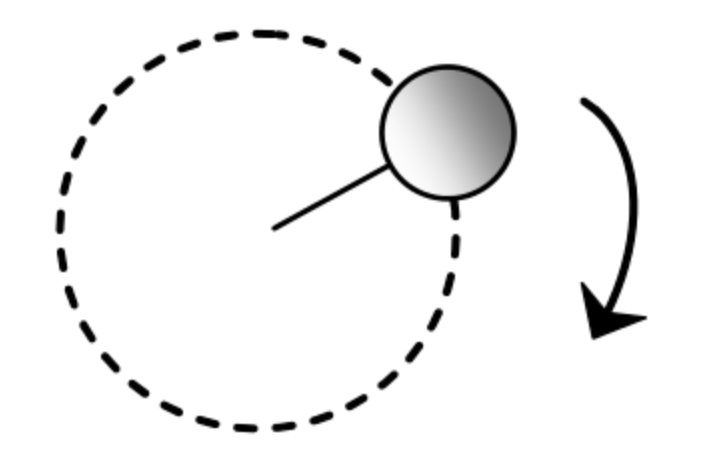
\includegraphics[height=0.5in]{circleball.png}
	\end{center}A ball is connected to a string and is moving in a circle, as shown in the diagram.  If the string were suddenly cut when the ball was in the position shown in the diagram, how would the ball move immediately after the string was cut?
\choice{Directly to the right}
\choice{directly to the left}
\choice{to the left and up}
\choice{to the right and down}

\end{question}

\begin{question}
	Alyssa gets on the tilt-a-whirl at Western Playland.  The tilt-a-whirl has a radius of 7m and has a tangential velocity of 12 m/s.  If Alyssa has a mass of 80 kg, what is the centripetal force that acts on her?  
	\choice{19.592 N}
	\choice{137.143 N}
	\choice{1645.71 N}
	\choice{11520 N}

\end{question}

\begin{question}
	\begin{center}
		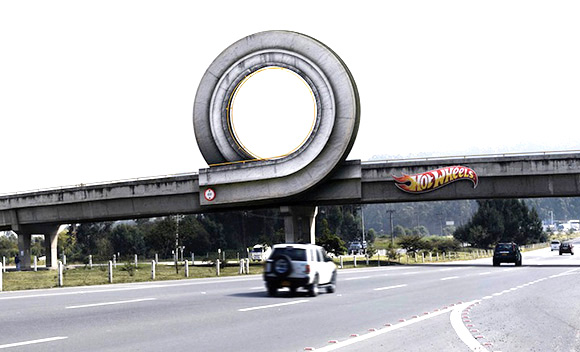
\includegraphics[height=1in]{hotwheels.png}
	\end{center}
Abby wants to drive her car around a loop, as seen in the picture.  If the radius of the loop is 35m and the mass of her car is 1000 kg, how fast would she need to go to make it around the loop?
\choice{0.529 m/s}
\choice{1.89 m/s}
\choice{18.520 m/s}
\choice{343 m/s}




\end{question}



\begin{question}
	 An object is traveling in a circle.  If the radius is doubled and all other variables stay the same, the centripetal force is - 
\choice{halved}
\choice{the same}
\choice{doubled}
\choice{quadrupled}
\end{question}


	
\begin{question}
	A car is driving on a circular track at a constant speed.  Which of the following statements is true?
	\choice{The car has a constant velocity.}
	\choice{The car's acceleration is 0 m/s\textsuperscript{2}}
	\choice{The magnitude of the force on the car is constant.}
	\choice{Gravity provides the centripetal force.}
	
\end{question}

\begin{question}
	The centripetal force acting on the space shuttle as it orbits Earth is equal to the shuttle’s
	\choice{inertia}
	\choice{velocity}
	\choice{momentum}
	\choice{weight}
	\end{question}

\begin{question}
The magnitude of the centripetal force acting on an object traveling in a horizontal, circular path will decrease if the 

\choice{radius of the path is increased}
\choice{mass of the object is increased}
\choice{direction of motion of the object is reversed}
\choice{speed of the object is increased}


\end{question}



\begin{question}
	The diagram below represents a mass, m, being 	swung clockwise at constant speed in a horizontal 	circle.
\begin{center}
	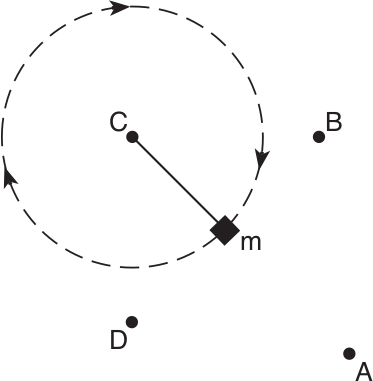
\includegraphics[height=1in]{centripetal1.png}
\end{center}
	At the instant shown, the centripetal force acting on mass m is directed toward point
	\choice{A}
	\choice{B}
	\choice{C}
	\choice{D}

\end{question}

\begin{question}
\begin{center}
	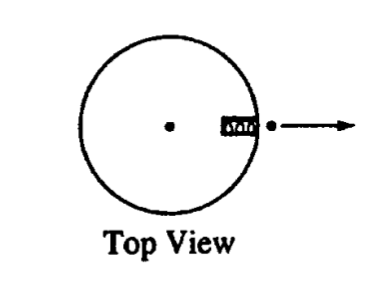
\includegraphics[height=1in]{disktop.png}
\end{center}
A compressed spring mounted on a disk can project a small ball. When the disk is not rotating, as shown in the top view above, the ball moves radially outward. The disk then rotates in a counterclockwise direction as seen from above, and the ball is projected outward at the instant the disk is in the position shown above. Which of the following best shows the subsequent path of the ball relative to the ground?
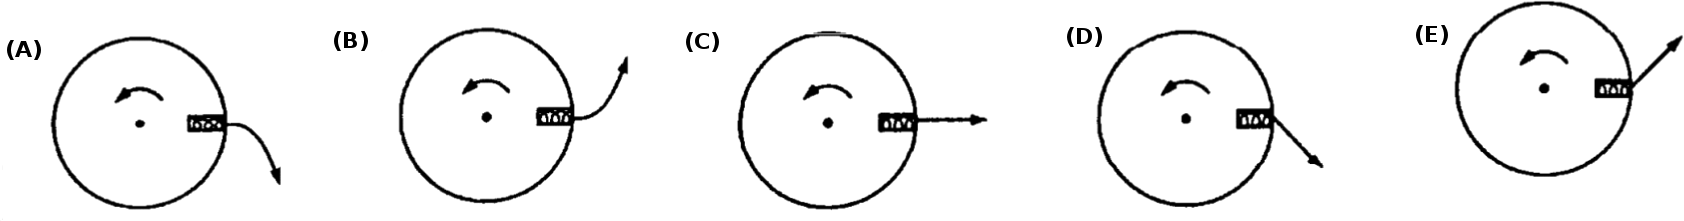
\includegraphics[height=.75in]{diskbottom.png}
\\ \hrule
	\end{question}


\begin{question}

	\begin{center}
		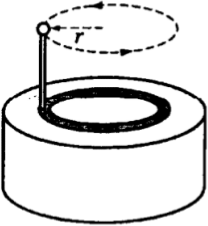
\includegraphics[height=1in]{circled.png}
	\end{center}
		
A steel ball supported by a stick rotates in a circle of radius r, as shown above. The direction of the net
force acting on the ball when it is in the position shown is indicated by which of the following?

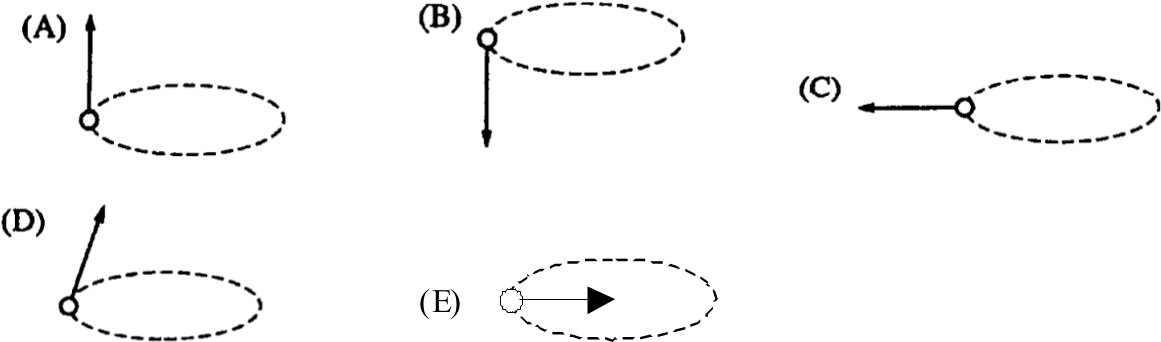
\includegraphics[height=1.75in]{circleda.png}
	\end{question}


\end{multiplechoice} 

\begin{shortanswer}[title={Free Response}]
	\begin{question}		
		The mass of the earth is 5.972 x 10\textsuperscript{24} kg, and the sun's gravity exerts a force of 3.593 x 10\textsuperscript{22} N on the Earth. Calculate the distance between the Earth and the Sun, assuming a circular orbit and an orbital speed of 3.00 x 10\textsuperscript{4} meters per second. 
		
		\vspace{2 in}
		\end{question}
	

	
	\end{shortanswer}




\end{document}


